\chapter{Implementácia programu}
V tejto kapitole sa budeme venovať niektorým významnejším črtám implementácie nášho programu
\section{Formát vstupu}
Evolučná história je tvorená postupnosťou riadkov, podobnej akú vidíme v tabulke  \ref{tab:vstup} . Prvý riadok opisuje počiatočný stav sekvencie.
Každý ďalší riadok, opisuje niektorú z udalostí, popísanú v sekcii \ref{evhist}.
\newline
Riadok obsahuje niekoľko reťazcov a čísel, oddelených medzerou alebo viacerými medzerami, pre lepšiu prehľadnosť.
\paragraph{Význam stĺpcov:}

\begin{description}

\item[Prvý stĺpec] je názov druhu, ktorého sa týka daný riadok.

\item[Druhý stĺpec] je id riadku.

\item[Tretí stĺpec] je id predchodcu, prvý riadok má špeciálneho predchodcu s hodnotou root.

\item[Štvrtý stĺpec] je čas, v ktorom sa daná udalosť odohrala. Koreň je v čase 0, a čas je rastúci.

\item[Piaty stĺpec] je skratka niektorej z udalostí, popísaných v sekcii \ref{evhist} alebo špeciálna udalosť. Root je udalosť slúžiaca na identifikáciu koreňa a leaf slúži na určenie času v ktorom sa daná vetva končí.

\item [Nasledujúce stĺpce] obsahujú postupnosť génov. Každý gén je celé číslo, pričom znamienko určuje jeho orientáciu. To znamená že gén 2 je rovnaký ako gén -2, iba opačne orientovaný.

\item [Znak \#] slúži ako ukončenie zoznamu génov.

\item[Zvyšné stĺpce], ktoré pre každý gén určujú poradie predka génu v predchodcovi jeho riadku. Ak tento gén nemá predchodcu, obsahuje riadok hodnotu -1.

\end{description}

\begin{table}[!htb]
\label{tab:vstup}
\begin{center}
\begin{tabular}{llllllll}
predok & e1 & root & 0 & root & 1 2 1 5 4 3 2 & \#  & -1 -1 -1 -1 -1 -1 -1 \\
predok & e2 & e1 &  0.05 & dup &  1 2 1 2 5 4 3 2 & \# & 0 1 2 1 3 4 5 6 \\
clovek & e3 & e2 &  0.12 & sp &   1 2 1 2 5 4 3 2 & \# & 0 1 2 3 4 5 6 7 \\
clovek & e4 & e3 &  0.13 & del & 1 2 1 2 4 3 2 & \# & 0 1 2 3 5 6 7 \\
clovek & e5 & e4 &  0.14 & ins & 1 2 1 6 7 2 4 3 2 & \# & 0 1 2 -1 -1 3 4 5 6 \\
clovek &  e6 & e5 &  0.2 & inv &  1 -1 -2 6 7 2 4 3 2 & \# & 0 2 1 3 4 5 6 7 8 \\
clovek & e7 & e6 &  0.25 & leaf & 1 -1 -2 6 7 2 4 3 2 & \# & 0 1 2 3 4 5 6 7 8 \\
simpanz & e8 & e2  & 0.12 & sp &  1 2 1 2 5 4 3 2 & \# & 0 1 2 3 4 5 6 7 \\
simpanz & e9 & e8 &  0.2 & leaf & 1 2 1 2 5 4 3 2 & \# & 0 1 2 3 4 5 6 7 \\
 \end{tabular}

\end{center}
\caption{Ukážka vymysleného vstupu v súčasnom formáte \cite{biowiki}}
\end{table}

\subsection{Navrhované zmeny}
\section{Návrh výstupu}
Výstupom programu je obrázok \ref{obr:tree} zakoreneného fylogenetický stromu , ktorý zobrazuje evolučné vzťahy medzi rôznymi druhmi na základe vzťahov medzi ich génmi.
X-ová os reprezentuje čas, v ktorom sa jednotlivé udalosti odohrali.
\newline
Strom druhov slúži ako pozadie pre gény.
\newline
Gény sú znázornené farebnými čiarami, ktoré idú vodorovne až kým nenastane nejaká udalosť.
\newline
Duplikácia je znázornená rozvetvením génu. 
\newline
Speciácia rozvetvením všetkých génov, a na rozdiel od duplikácie sa vetví aj strom druhov.
\newline 
Inzercia génu je znázornená ako pridanie novej čiary, na prislúchajúce miesto do stromu druhov.
\newline
Delécia je ukončenie čiary, ktorá znázorňuje gén.
\newline 
Inverzia je znázornená ako kríženie čiar preusporiadaných génov.
\newline 
Leaf je znázornení ako ukončenie stromu druhov a všetkých génov v tejto vetve.
\newline
Root je začiatok stromu druhov a aj všetkých génov, ktoré sa nachádzajú v počiatočnom predkovi.
\begin{figure}
\centerline{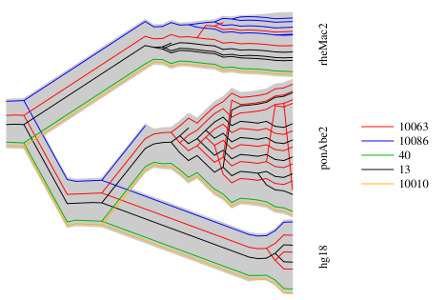
\includegraphics[width=1\textwidth]{images/DUP-tube-tree}}
\caption{Možný vzhľad fylogenetického stromu \cite{Vinar2010}}\label{obr:tree}
\end{figure}
\subsection{Možné zmeny}
Súčasný návrh vizualizácie nezobrazuje všetky informácie zo vstupu. Jedným z údajov, 
ktorý sa stráca je orientácia génu.
Tak isto z obrázku nieje zrejmé, v ktorom chromozóme sa gén nachádza.  